\section{Aufbau}
\begin{frame}
	\frametitle{System}
	Verwendung einer Speicherkarte zum speichern der Authentifizierungsdaten.\\
	Aufteilung in \textbf{Master} und \textbf{Terminal} um:
	\begin{itemize}
	\item<2-> Aufgaben Verteilung
	\item<3-> Besondere Sicherung der Master Unit
	\end{itemize}
\end{frame}

\begin{frame}
	\frametitle{Grundaufbau}
	\begin{center}
		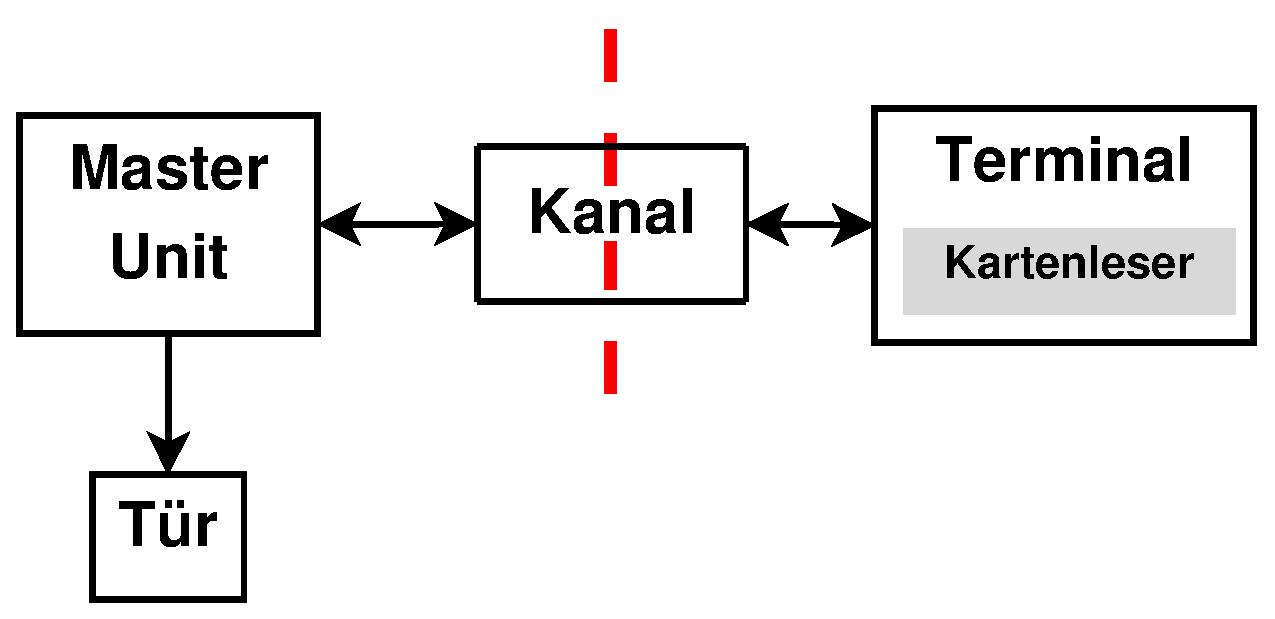
\includegraphics[width=210px]{grundaufbau}
	\end{center}
\end{frame}

\begin{frame}
	\frametitle{Master Unit}
	\begin{itemize}
		\item<2-> Speicherung der Datenbank
		\item<3-> Authentifizierung der Nutzer
		\item<4-> Löschung der Schlüssel \& Datenbank bei physikalischen Angriffen
		\item<5-> Unterbrechungsfrei Stromversorgung (USV)
	\end{itemize}
\end{frame}

\begin{frame}
	\frametitle{Terminal/Panel}
	\begin{itemize}
		\item<2-> Weitergabe der Kartendaten
		\item<3-> Ein- und Ausgabe \small{(Master Unit \texttt{<->} Mensch)}
		\item<4-> Löschung des Schlüssels bei physikalischen Angriffen
	\end{itemize}
\end{frame}

\begin{frame}
	\frametitle{Kanal (logisch)}
	Verbindung über kryptografisch sicheren Kanal
	\begin{itemize}
		\item<2-> Integrität
		\item<3-> Authentizität
		\item<4-> Vertraulichkeit
	\end{itemize}
\end{frame}

\begin{frame}
	\frametitle{Kanal (physikalisch)}
	Galvanische Trennung zwischen Master Unit und Panel, z.B.
	\begin{itemize}
		\item<2-> Funk
		\item<3-> LWL / Optokoppler
	\end{itemize}
\end{frame}

\begin{frame}
	\frametitle{Speicherkarte}
	Speicherung der zur Authentifierung nötigen Daten (z.B. Ticket).
	\begin{itemize}
		\item<2-> Chipkartenformat: handlich
		\item<3-> Günstig: < 1 \euro{} pro Stück
		\item<4-> Transparent: Daten können von jedem nach belieben ausgelesen werden.
	\end{itemize}
\end{frame}